\documentclass{beamer}
%\usepackage{amsfonts,amsmath,oldgerm}
\usetheme{sintef}
\usepackage{booktabs}
\usepackage{verbatim}
\usepackage{physics}
\usepackage{listings}
\usepackage{tikz} % Allows to draw custom shapes
\usepackage{tikzpagenodes}
\usepackage{appendixnumberbeamer}
\usepackage{pgfplots}
\pgfplotsset{compat=1.18}
\definecolor{listingkeywords}{rgb}{0.0, 0.5, 0.0}
\definecolor{listingidentifiers}{rgb}{0, 0, 0}
\definecolor{listingcomments}{rgb}{0.25, 0.5, 0.5}
\definecolor{listingstrings}{rgb}{0.73, 0.13, 0.13}
\definecolor{listingnumbers}{rgb}{0.25, 0.25, 0.25}
\lstdefinestyle{kaolst}{
	aboveskip=0.7\topskip,
	belowskip=0.1\topskip,
	basicstyle=\scriptsize\ttfamily,
	commentstyle=\color{listingcomments}\itshape,
	keywordstyle=\color{listingkeywords}\bfseries,
	numberstyle=\scriptsize\color{listingnumbers}\ttfamily,
	stringstyle=\color{listingstrings},
	identifierstyle=\color{listingidentifiers},
    morekeywords={for,set,end,each},
	breakatwhitespace=false,
	breaklines=true,
	captionpos=t,
	keepspaces=true,
	showspaces=false,
	showstringspaces=false,
	showtabs=false,
	numbers=none,
	numbersep=1em,
	%frame=lines,
	frame=none,
	framerule=.7pt,
	tabsize=4,
	defaultdialect=[LaTeX]Tex,
}
\lstdefinestyle{kaolstplain}{
	aboveskip=0.6\topskip,
	belowskip=-0.1\topskip,
	basicstyle=\scriptsize\ttfamily,
	commentstyle=\color{listingcomments}\itshape,
	keywordstyle=\color{listingkeywords}\bfseries,
	numberstyle=\scriptsize\color{listingnumbers}\ttfamily,
	stringstyle=\color{listingstrings},
	identifierstyle=\color{listingidentifiers},
	breakatwhitespace=false,
	breaklines=true,
	captionpos=t,
	keepspaces=true,
	showspaces=false,
	showstringspaces=false,
	showtabs=false,
	numbers=none,
	frame=none,
	tabsize=4,
	defaultdialect=[LaTeX]Tex,
}



\newcommand{\testcolor}[1]{\colorbox{#1}{\textcolor{#1}{test}}~\texttt{#1}}

%\usefonttheme[onlymath]{serif}

\titlebackground*{assets/background_old}

\newcommand{\hrefcol}[2]{\textcolor{cyan}{\href{#1}{#2}}}

\title{Neural Networks as Quantum States}
\subtitle{NNs in Quantum Many-Body Problems}
\course{Deep Learning con Applicazioni}
\author{\href{mailto:stefano.lonardoni1@studenti.unimi.it}{Stefano Lonardoni}}

\begin{document}
\maketitle

\begin{frame}{Introduction}
\framesubtitle{Neural Networks as Quantum States}
\begin{itemize}
	\item Quantum-many-body problems feature an exponential Hilbert-space growth
	\item Traditional variational ansätze reduce complexity sactificing correlation and entanglement
	\item Neural-network quantum states can offer expressivity with a compact set of parameters
\end{itemize}

\textbf{Neural Networks can represent ground states for a many-body quantum system}\footnote{Giuseppe Carleo, Matthias Troyer, Solving the quantum many-body problem with artificial neural networks. \textit{Science} 355, 602-606 (2017)}

\end{frame}

\begin{chapter}[assets/background_negative]{}{Project Outline}
\framesubtitle{Find the Ground State}
\begin{itemize}
	\item Restricted Boltzmann Machine as a neural network
	\item Sample configurations from RBM
	\item Train RBM to find the ground state
\end{itemize}
\end{chapter}

\begin{frame}{Restricted Boltzmann Machine}
\framesubtitle{Generative Model}
\begin{columns}
\begin{column}{0.68\textwidth}
\begin{itemize}
    \item Learns $p(\vec{\sigma})$ of the input data $\vec{\sigma}$
    \item Two layers: $N$ visible and $M$ hidden
    \item Parameters $\mathcal{W}$: weights $W_{ij}$ and biases $b_i$, $c_j$
\end{itemize}
\end{column}
\begin{column}{0.3\textwidth}
\begin{center}
    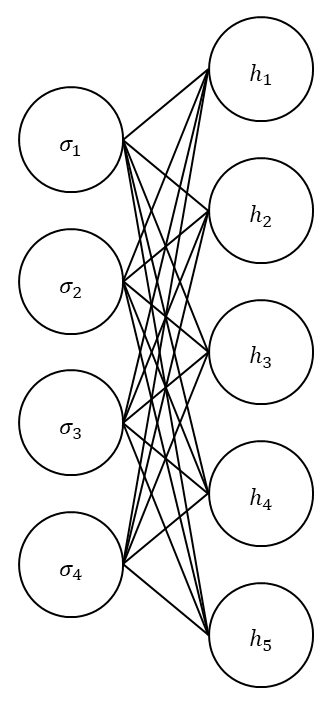
\includegraphics[height=\textheight]{images/rbm.png}
\end{center}
\end{column}
\end{columns}
\end{frame}

\begin{frame}{Restricted Boltzmann Machine}
\framesubtitle{Probability Distribution}
Internal Energy:
$$E(\vec{\sigma}, \vec{h}) = -\sum_{i} b_i \sigma_i - \sum_{j} c_j h_j - \sum_{i,j} W_{ij} \sigma_i h_j$$

Probability Distribution:
$$p(\vec{\sigma}, \vec{h}) = \frac{1}{Z} e^{-E(\vec{\sigma}, \vec{h})}$$

where $Z$ is the partition function:
$$Z = \sum_{\vec{\sigma}, \vec{h}} e^{-E(\vec{\sigma}, \vec{h})}$$
\end{frame}

\begin{frame}{Restricted Boltzmann Machine}
\framesubtitle{Application to Quantum States}
Considering a spin configuration $\vec{\sigma}$ and a set of parameters $\mathcal{W}$:
$$\psi\left( \vec{\sigma}, \mathcal{W} \right) = e^{\sum_{i} b_i \sigma_i + \sum_{j} c_j h_j + \sum_{i,j} W_{ij} \sigma_i h_j}$$

With no intra-layer connections:
$$\psi\left( \vec{\sigma}, \mathcal{W} \right) = e^{\sum_{i} b_i \sigma_i} \times \prod_{j=1}^{M} {2 cosh\left[c_j + \sum_{i} W_{ij} \sigma_i\right]}$$

From the RBM we can sample configurations $\vec{\sigma}$.

\end{frame}

\begin{frame}{Training}
\framesubtitle{Reinforcement Learning}
Update parameters $\mathcal{W}$ towards energy minimum.

$$
E_0 \;\le\;
\frac{\bra{\psi_{\mathcal{W}}} \hat H \ket{\psi_{\mathcal{W}}} }
	{\bra{\psi_{\mathcal{W}}} \ket{\psi_{\mathcal{W}}}}
$$
\vskip1\baselineskip

The parameters $\mathcal{W}$ are optimized using a gradient descent method\footnote{Becca F, Sorella S. \textit{Quantum Monte Carlo Approaches for Correlated Systems}. Cambridge University Press; 2017}:
\begin{itemize}
	\item Variational Monte Carlo (VMC)
	\item Stochastic Reconfiguration (SR)
\end{itemize}

\end{frame}

\begin{frame}{Training}
\framesubtitle{Variational Monte Carlo}
We can compute the gradients:
\begin{equation*}
\begin{aligned}
    \nabla_{\mathcal{W}} \left(E\right) &= \nabla_{\mathcal{W}} \langle E_{\text{loc}} \rangle \\
    &= \langle E_{\text{loc}} \nabla_{\mathcal{W}} log(p_{\psi}) \rangle \\
    &= 2 \mathfrak{R} \left[ \langle E_{\text{loc}} \nabla_{\mathcal{W}} log(\psi) \rangle - \langle E_{\text{loc}} \rangle \langle \nabla_{\mathcal{W}} log(\psi) \rangle \right]
\end{aligned}
\end{equation*}
And consequently update the parameters:
$$\Delta \mathcal{W} = - \eta \nabla_{\mathcal{W}} \left(E\right)$$
\end{frame}

\begin{frame}{Training}
\framesubtitle{Stochastic Reconfiguration}
Parameters evolution in the variational space:
$$\Delta \mathcal{W} = - \eta \mathbf{S}^{-1} \vec{F}$$
where $\mathbf{S}^{-1}$ is the pseudo-inverse of the covariance matrix:
$$\mathbf{S}_{ij} = \langle O_i^{*} O_j \rangle - \langle O_i^{*} \rangle \langle O_j \rangle$$
and $\vec{F}$ is the force vector:
$$F_i = \langle O_i^{*} E_{\text{loc}} \rangle - \langle O_i^{*} \rangle \langle E_{\text{loc}} \rangle$$
where $O_i$ are the local operators defined as:
$$O_i = \frac{\partial log\left(\psi\left( \vec{\sigma}, \mathcal{W} \right)\right)}{\partial W_{ij}}$$

\end{frame}

\begin{chapter}[assets/background_negative]{}{Code Implementation}
\begin{itemize}
    \item RBM
    \item Sampler
    \item Hamiltonian
    \item Optimizers
\end{itemize}
\end{chapter}

\begin{frame}[fragile]{Code Implementation}
\framesubtitle{Project Structure}
\begin{itemize}
	\item \lstinline[style=kaolstplain]|RBM| class computes $log(\psi)$
	\item Sampler(s) sample configurations from the RBM
	\item Hamiltonian class computes local energies
	\item \lstinline[style=kaolstplain]|QOptimizer| class implements the optimizers
\end{itemize}
\end{frame}

\begin{frame}[fragile]{Code Implementation}
\framesubtitle{RBM}

Custom \lstinline[style=kaolstplain]|tf.module| implementing the RBM.
\vskip1\baselineskip

Weights and biases are initialized randomly as complex values:
\begin{lstlisting}[language=Python, style=kaolstplain]
self.W = tf.Variable(
	tf.random.normal([self.N_visible, self.N_hidden], dtype=tf.complex64)
)
self.b = tf.Variable(tf.random.normal([self.N_visible], dtype=tf.complex64))
self.c = tf.Variable(tf.random.normal([self.N_hidden], dtype=tf.complex64))
\end{lstlisting}

$$\psi\left(\vec{\sigma}, \mathcal{W}\right) = e^{\sum_{i} b_i \sigma_i} \times \prod_{j=1}^{M} {2 cosh\left[c_j + \sum_{i} W_{ij} \sigma_i\right]}$$

\end{frame}

\begin{frame}[fragile]{Code Implementation}
\framesubtitle{RBM - Logarithm of the Wave Function}

\begin{center}
    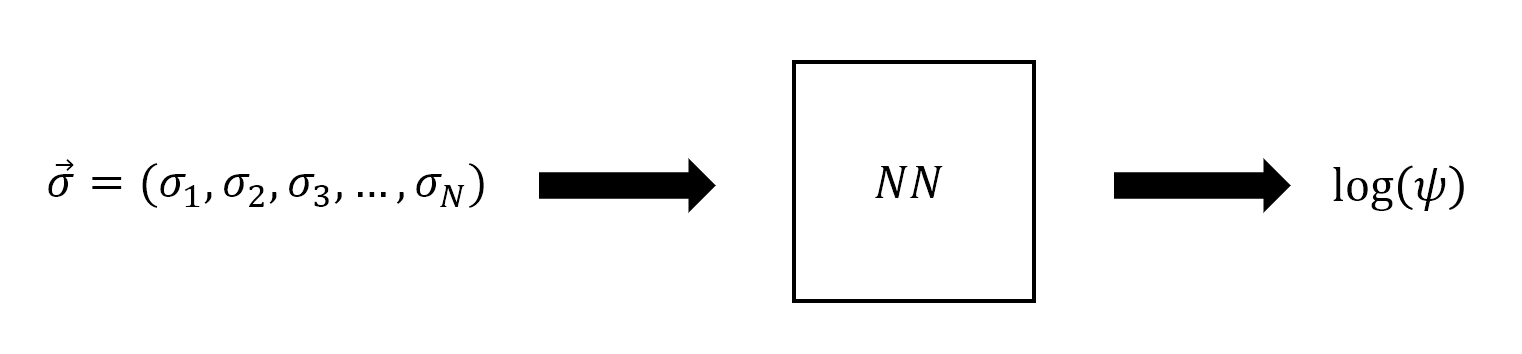
\includegraphics[height=2cm]{images/rbm_usage.png}
\end{center}

$$log\left(\psi\right) = \sum_{i} b_i \sigma_i + \sum_{j=1}^{M} log\left[{2 cosh\left(c_j + \sum_{i} W_{ij} \sigma_i\right)} \right]$$

\end{frame}

\begin{frame}[fragile]{Code Implementation}
\framesubtitle{RBM - Logarithm of the Wave Function}
\begin{columns}
\begin{column}{0.6\textwidth}
\begin{lstlisting}[language=Python, style=kaolstplain]
sum_visible = tf.reduce_sum(
	a * spins, axis=1
)
w_h = b + tf.matmul(spins, W)
sum_hidden = tf.reduce_sum(
	tf.math.log(2.0 * (
		tf.math.cosh(b + tf.matmul(spins, W))
	)),axis=1
)
return sum_visible + sum_hidden
\end{lstlisting}
\end{column}
\begin{column}{0.38\textwidth}
$$\sum_{i} b_i \sigma_i$$
$$\sum_{j=1}^{M} log\left[{2 cosh\left(c_j + \sum_{i} W_{ij} \sigma_i\right)} \right]$$
\end{column}
\end{columns}

\end{frame}


\begin{frame}[fragile]{Code Implementation}
\framesubtitle{Sampler}

Samples configurations from the RBM.

\begin{itemize}
    \item \textbf{Metropolis-Hastings} Random Walk using \textit{TensorFlow Probability}
    \item \textbf{Gibbs sampling} Double-step method to sample visible and hidden variables
\end{itemize}

Provides batches of configurations. Example:
\begin{center}
\begin{lstlisting}[language=Python, style=kaolstplain]
>>> sam.sample(rbm)
<tf.Tensor: shape=(5, 4), dtype=float32, numpy=
array([[0., 0., 0., 0.],
       [1., 1., 1., 0.],
       [0., 0., 1., 0.],
       [0., 0., 0., 0.],
       [0., 0., 0., 1.]], dtype=float32)>
\end{lstlisting}	
\end{center}

\end{frame}

\begin{frame}[fragile]{Code Implementation}
\framesubtitle{Hamiltonian - 1D Ising}

Simple 1D Ising Hamiltonian:
$$ H = -J \sum_{i} \sigma_{i} \sigma_{i+1} - h \sum_{i} \sigma_{i} $$

Provides \lstinline[style=kaolstplain]|local_energy(samples)| which computes $E_{\text{loc}}$ for each configuration $\vec{\sigma}$.

\end{frame}

\begin{frame}[fragile]{Code Implementation}
\framesubtitle{Optimizers}
Leverage \lstinline[style=kaolstplain]|tf.GradientTape| to compute gradients of $log\left(\psi\right)$
\begin{lstlisting}[language=Python, style=kaolstplain]
with tf.GradientTape() as tape:
	log_psi = self.wave_function.log_psi(samples)
grad_log_psi = tape.jacobian(log_psi, self.wave_function.trainable_variables)
\end{lstlisting}
\vskip1\baselineskip

VMC and SR methods obtain parameters update in different ways.
\vskip1\baselineskip

Update the parameters of the wave function in the same way:
\begin{lstlisting}[language=Python, style=kaolstplain]
for grad_val, var in grads_vars:
	var.assign_sub(self.learning_rate * grad_val)
\end{lstlisting}
\end{frame}

\begin{frame}[fragile]{Code Implementation}
\framesubtitle{Optimizers - VMC}
The VMC approach computes the variational increments as follows:
\begin{lstlisting}[language=Python, style=kaolstplain]
mean_energy = tf.reduce_mean(local_energies)
for grad_i in grad_log_psi:
	loc_grad = e_loc * grad_i
	grad_energy = tf.reduce_mean(loc_grad, axis=0)
	grad_log_psi_mean = tf.reduce_mean(grad_i, axis=0)

	vmc_grad = 2.0 * tf.math.real(
		grad_energy - mean_energy * grad_log_psi_mean
	)
	gradients.append(vmc_grad)
\end{lstlisting}
\end{frame}

\begin{frame}[fragile]{Code Implementation}
\framesubtitle{Optimizers - Stochastic Reconfiguration}
The SR approach computes the variational increments as follows:
\begin{lstlisting}[language=Python, style=kaolstplain]
O_mean = tf.reduce_mean(O, axis=0)
# compute covariance matrix / QGT
O_O = tf.matmul(O_mean, O_mean, transpose_a=True)
S = O_O / norm
# compute force vector
mean_energy = tf.reduce_mean(local_energies)
F_vec = (
	tf.reduce_mean(local_energies[:, None] * O, axis=0) - mean_energy * O_mean
)
# solve for delta
P = tf.shape(S)[0]
S_reg = S + self.epsilon * tf.eye(P, dtype=S.dtype)
# dW = S^{-1} F
gradients = tf.linalg.solve(S_reg, tf.expand_dims(F_vec, 1))
\end{lstlisting}
\end{frame}

\begin{chapter}[assets/background_negative]{}{Results}
\end{chapter}

\begin{frame}{Results}
\framesubtitle{1D Ising Model - 16 spins}
Using $J = 1.0$ and $h=0.5$
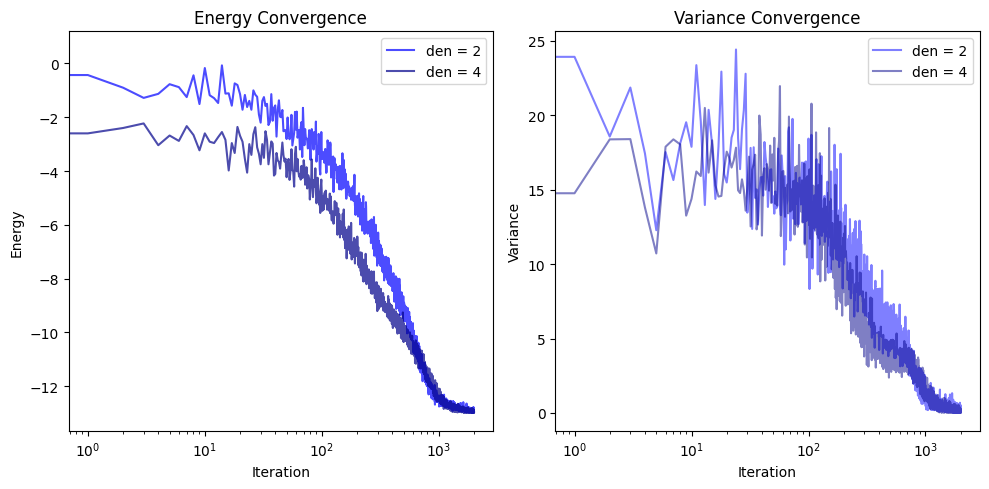
\includegraphics[height=6cm]{images/16spin_history_j1.png}
\end{frame}

\begin{frame}{Results}
\framesubtitle{Weights for $den = 1$}
\begin{center}
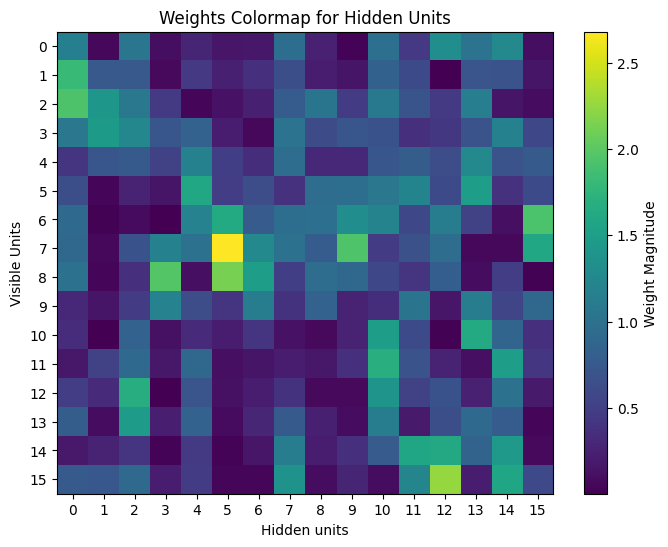
\includegraphics[height=6cm]{images/16spin_den1_j1.png}
\end{center}
\end{frame}

\begin{frame}{Results}
\framesubtitle{Weights for $den = 2$}
\begin{center}
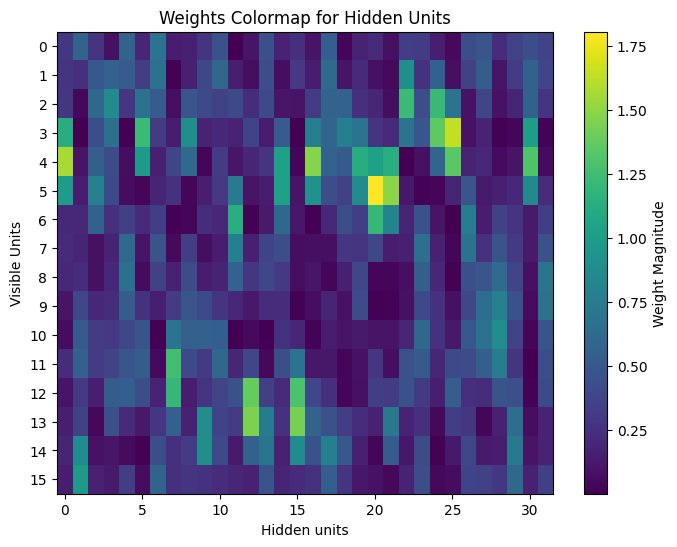
\includegraphics[height=6cm]{images/16spin_den2_j1.png}
\end{center}
\end{frame}

\begin{frame}{Results}
\framesubtitle{Weights for $den = 4$}
\begin{center}
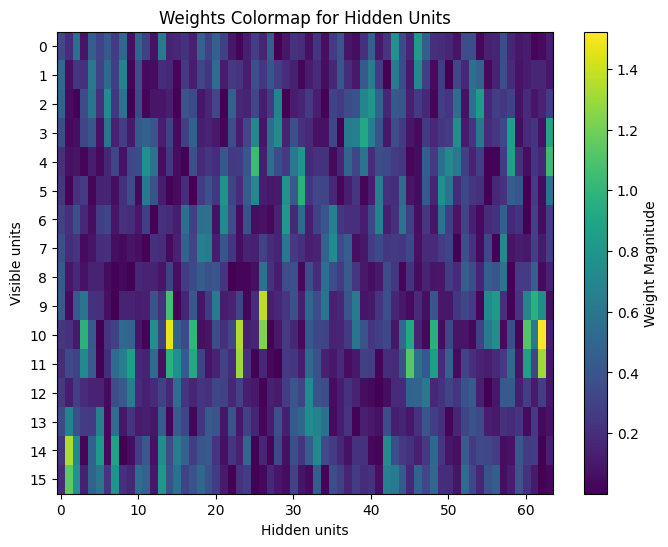
\includegraphics[height=6cm]{images/16spin_den4_j1.png}
\end{center}
\end{frame}

\begin{frame}{Results}
\framesubtitle{1D Ising Model - 16 spins}
Using $J = -1.0$ and $h=0.5$
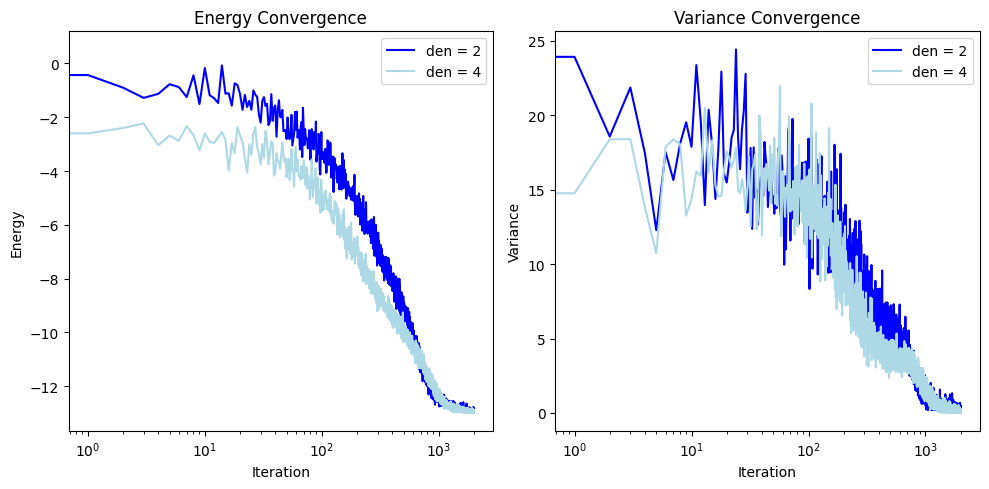
\includegraphics[height=6cm]{images/16spin_history_jm1.png}
\end{frame}

\begin{frame}{Results}
\framesubtitle{Weights for $den = 2$}
\begin{center}
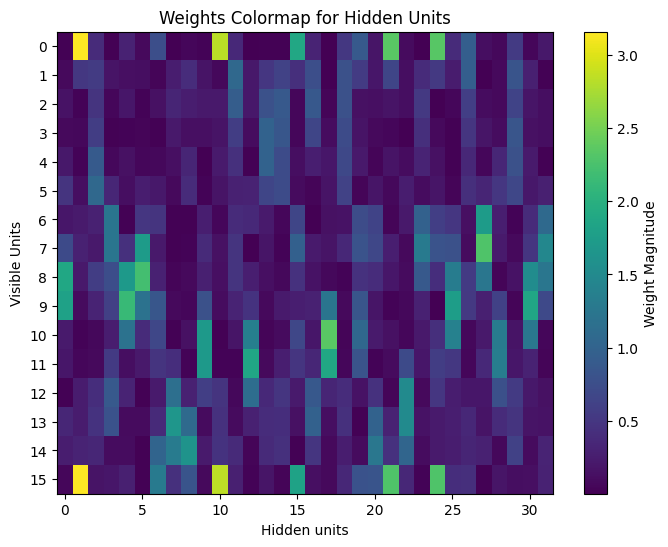
\includegraphics[height=6cm]{images/16spin_den2_jm1.png}
\end{center}
\end{frame}

\begin{frame}{Results}
\framesubtitle{Weights for $den = 4$}
\begin{center}
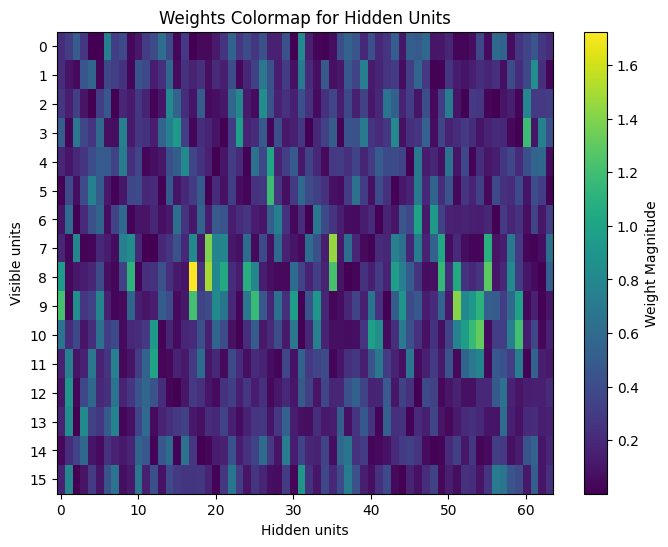
\includegraphics[height=6cm]{images/16spin_den4_jm1.png}
\end{center}
\end{frame}

\begin{frame}{Further Work}
\framesubtitle{Optimization and Extensions}
\begin{columns}
\begin{column}{0.5\textwidth}
\begin{itemize}
	\item Extend to 2D systems
	\item Other neural networks (FFNN, CNN)
	\item Unitary (and non) dynamics
\end{itemize}
\end{column}
\begin{column}{0.5\textwidth}
\begin{itemize}
	\item Efficient SR update (single parameter updates)
	\item Change tensor framework (JAX, ...)
\end{itemize}
\end{column}
\end{columns}
\end{frame}

\begin{frame}{Other Works}
\begin{columns}
\begin{column}{0.6\textwidth}
\textbf{NetKet}: The Machine-Learning toolbox for Quantum Physics
\end{column}
\begin{column}{0.3\textwidth}

\includegraphics[width=\textwidth]{images/netket.png}
\end{column}
\end{columns}
\end{frame}

\begin{frame}{References}

\end{frame}

\backmatter

\appendix


\begin{chapter}[assets/background_negative]{}{Appendix}
\end{chapter}

\begin{frame}{Appendix}
\framesubtitle{Probabilities for the RBM}

Thanks to no intra-layer connections, we can factorize the joint probability:

\begin{columns}[t]
	\begin{column}{0.48\textwidth}
		$$ p(\vec{\sigma} \mid \vec{h}) = \prod_{i} p(\sigma_i \mid \vec{h}) $$
	\end{column}
	\begin{column}{0.48\textwidth}
		$$ p(\vec{h} \mid \vec{\sigma}) = \prod_{j} p(h_j \mid \vec{\sigma}) $$
	\end{column}
\end{columns}
where:
$$ p(\sigma_i | h) = \sigma\left(b_i + \sum_{j} W_{ij} h_j\right) $$
$$ p(h_j | \sigma) = \sigma\left(c_j + \sum_{i} W_{ij} \sigma_i\right) $$
where $\sigma(x) = \frac{1}{1 + e^{-x}}$ is the logistic or sigmoid function.

\end{frame}

\begin{frame}{Appendix}
\framesubtitle{Local operators for the RBM}
Explicit form of the partial derivatives of $log\left(\psi\right)$


\end{frame}

\begin{frame}[fragile]{Appendix}
\framesubtitle{Metropolis-Hastings and MCMC sampling}
Propose a single bit flip, and accept it with the Metropolis criterion:
$$\alpha = \min\left(1, \frac{p(\sigma')}{p(\sigma)}\right)$$
where $\sigma'$ is the proposed state and $\sigma$ is the current state.
\vskip1\baselineskip

Uses the \lstinline[style=kaolstplain]|tfp.mcmc| module for efficient sampling.
\begin{itemize}
	\item Requires target $log(p)$
	\item Requires new state proposal
\end{itemize}

\end{frame}

\begin{frame}[fragile]{Appendix}
\framesubtitle{Gibbs sampling}
We can sample the visible and hidden variables in a double-step Gibbs sampling:
\begin{lstlisting}[language=Python, style=kaolstplain]
def sample(self, wave_function):
	v = tf.cast(self.current_state, tf.float32)
	for _ in range(self.k):
		v_complex = tf.cast(v, wave_function.W.dtype)
		v_W = tf.matmul(v_complex, wave_function.W)
		p_h = tf.sigmoid(tf.math.real(wave_function.b + v_W))
		h = tf.cast(tf.random.uniform(tf.shape(p_h), dtype=tf.float32) < p_h, tf.float32)
		h_complex = tf.cast(h, wave_function.W.dtype)
		h_Wt = tf.matmul(h_complex, tf.transpose(wave_function.W))
		p_v = tf.sigmoid(tf.math.real(wave_function.a + h_Wt))
		v = tf.cast(tf.random.uniform(tf.shape(p_v), dtype=tf.float32) < p_v, tf.float32)
	self.current_state.assign(tf.cast(v, tf.int32))
return v
\end{lstlisting}
\end{frame}

\end{document}
